\documentclass{rspublic}   

%------------------------------------------------------------------------- 
% take the % away on next line to produce the final camera-ready version 
%\pagestyle{empty}

%\usepackage[utf8]{inputenc}
\usepackage{graphicx}
\usepackage{url}
\usepackage{float}
\usepackage{times}    
\usepackage{multirow}    
\usepackage{listings}   
\usepackage{times}     
\usepackage{paralist}    
\usepackage{wrapfig}    
\usepackage[small,it]{caption}
\usepackage{multirow}
\usepackage{ifpdf}   
\usepackage{subfigure} 

                    
%Bibliography                     
\usepackage{natbib}   

\usepackage{listings}
\usepackage{keyval}  
\usepackage{color}
\definecolor{listinggray}{gray}{0.95}
\definecolor{darkgray}{gray}{0.7}
\definecolor{commentgreen}{rgb}{0, 0.4, 0}
\definecolor{darkblue}{rgb}{0, 0, 0.4}
\definecolor{middleblue}{rgb}{0, 0, 0.7}
\definecolor{darkred}{rgb}{0.4, 0, 0}
\definecolor{brown}{rgb}{0.5, 0.5, 0}



\title[Efficient Replica-Exchange Simulations on
  Large-Scale Production Infrastructure]{Efficient Replica-Exchange Simulations on
  Large-Scale Production Infrastructure}

\author[Thota, Luckow, Jha]{
  Abhinav Thota$^{1,2}$, Andr\'e Luckow$^{1}$ and Shantenu Jha$^{1,2,3}$\\
  \small{\emph{$^{1}$Center for Computation \& Technology, Louisiana State University, Baton Rouge, LA 70803, USA}}\\
  \small{\emph{$^{2}$Department of Computer Science, Louisiana State
      University, Baton Rouge, LA 70803, USA}}\\
  \small{\emph{$^{3}$e-Science Institute, Edinburgh EH8 9AA, UK}}\\
}

%\date{}

\def\acknowledgementname{Acknowledgements}
\newenvironment{acknowledgement}%
{\section*{\acknowledgementname}%
\parindent=0pt%
}

\newif\ifdraft
\drafttrue
\ifdraft
\newcommand{\jhanote}[1]{ {\textcolor{red} { ***shantenu: #1 }}}
\newcommand{\alnote}[1]{ {\textcolor{blue} { ***andre: #1 }}}
\newcommand{\athotanote}[1]{ {\textcolor{green} { ***athota: #1 }}}
\else
\newcommand{\alnote}[1]{}
\newcommand{\athotanote}[1]{}
\newcommand{\jhanote}[1]{}
\fi

\newcommand{\I}[1]{\textit{#1}}
\newcommand{\B}[1]{\textbf{#1}}
\newcommand{\T}[1]{\texttt{#1}}

\newcommand{\glidein}[1]{Glide-In }  
\newcommand{\replicaagent}[1]{Replica-Agent }         
\newcommand{\remanager}[1]{RE-Manager }

\begin{document} 


\maketitle    

\begin{abstract}{Replica-Exchange, SAGA, Large-Scale, Production}  

  Developing applications that are able to orchestrate heterogeneous
  resources across distributed resources is a complex
  task. Inevitably, the design and development of an application is
  influenced and constrained by the programming systems and the
  infrastructure it is developed against. Breaking this coupling
  between the development and the underlying infrastructure, to enable
  applications to be flexible (across infrastructure), extensible (to
  new methods of communication and coordination) and scalable is an
  important design objective of both logically and physically
  distributed applications.  In this work, we focus on the
  Replica-Exchange (RE) Methods which represent a class of algorithms
  that involve a large number of loosely-coupled ensembles. RE
  simulations are used to understand physical phenomena Ð ranging from
  protein folding dynamics to binding affinity calculations.  In this
  work, we develop a flexible, extensible and scalable implementation
  of RE that can utilise a range of infrastructure concurrently
  \jhanote{(and autonomically/adaptively): Do we?}, that supports
  different coordination mechanisms (publish-subscribe \jhanote{do
    we?}, centralised notification), different replica pairing
  mechanisms (synchronous versus asynchronous) and thereby different
  variants of the RE algorithm. We implement and demonstrate how a
  flexible and robust implementation enables the efficient use of a
  broad range of infrastructure.

% Developing applications that are able to orchestrate heterogeneous
% resources across distributed resources is a complex task. Inevitably,
% the design and development of an application is influenced and
% constrained by the programming systems and the infrastructure it is
% developed against. Breaking this coupling between the development and
% the underlying infrastructure, to enable applications to be flexible
% (across infrastructure), extensible (to new methods of communication
% and coordination) and scalable is an important design objective of
% distributed applications both logically distributed and physically
% distributed.  In this work, we focus on the Replica-Exchange (RE)
% Methods which represent a class of algorithms that involve a large
% number of loosely-coupled ensembles. RE simulations are used to
% understand physical phenomena Ð ranging from protein folding dynamics
% to binding affinity calculations.  In this work, we develop a
% flexible, extensible and scalable implementation of RE that can
% utilise a range of infrastructure concurrently (and
% autonomically/adaptively), that supports different coordination
% mechanisms (publish/subscribe, centralized notification), different
% replica pairing mechanisms (synchronous versus asynchronous) and
% thereby different variants of the RE algorithm. We implement and
% demonstrate how a flexible and robust implementation enables the
% efficient use of a broad range of infrastructure.

\end{abstract}

\jhanote{please use \citep{} and not \cite{}}

\section{Introduction}
Developing applications that are able to orchestrate heterogeneous
resources across distributed resources is a complex task.  Inevitably,
the design and development of an application is influenced and
constrained by the programming systems and the infrastructure it is
developed against. Breaking this coupling between the development and
the underlying infrastructure, to enable applications to be flexible
(across infrastructure), extensible (to new methods of communication
and coordination) and scalable is an important design objective of
distributed applications -- both logically distributed and physically
distributed.

In this work, we focus on the Replica-Exchange
(RE)~\citep{hansmann,Sugita:1999rm} methods -- which represent a class
of algorithms that involve a large number of loosely-coupled
ensembles.  RE simulations are used to understand physical phenomena
-- ranging from protein folding dynamics to binding affinity
calculations. Most RE implementations are either infrastructure
specific (Woods et al. 2005) or, if using multiple distributed
resources, they require prior co-scheduling (Manos et
al. 2008). ~\citep{Luckow:2008fp} takes it to the next level and is an
example of adaptive RE simulations on production-level grid resources,
while ~\citep{parashar_arepex} is an example of \emph{asynchronous} RE
simulations, which is based on
CometG~\citep{Li:2005:CSC:1090948.1091381}, a decentralised
computational infrastructure for Desktop Grid environments.

We develop a flexible, extensible and scalable implementation of RE
that can utilize a range of infrastructure concurrently that supports
different coordination mechanisms (publish-subscribe, centralised
notification), different replica pairing mechanisms (synchronous
versus asynchronous) and thereby different variants of the RE
algorithm.  Application formulations that are scalable while being
flexible and extensible are better suited to using the diverse range
of traditional and hybrid infrastructure (e.g., Grid-Cloud and
heterogeneous resources).  

Along with application formulations that facilitate the flexible
utilisation of a range of infrastructure, it is imperative to have the
correct run-time abstractions that support flexible deployment of
these applications.  Consequently, we utilize a flexible pilot-job
implementation (SAGA BigJob) to support the execution of our
formulations.  We implement and demonstrate how a flexible and robust
implementation enables the efficient use of a broad range of
infrastructure. We compare and analyze the performance of the
different RE models (synchronous and asynchronous) when we scale-up to
256 replicas and scale-out to 4 machines. We present results using
which the reader can understand which model of RE is most suited for a
particular set of resources (distributed, local etc.,)

The rest of the paper is organized as follows. Section II sketches out
the different RE algorithms that we investigate. Section III outlines
the architecture of the SAGA BigJob and how it supports the dynamic
execution of multiple replicas (ensembles). In Section IV, we present
the implementation details of the RE algorithms and understand
the primary determinants of performance; we also present
an approximate mathematical model for the different algorithms.
% We also present
% different implementations of the asynchronous RE algorithm. 
In Section V, we describe the experiments performed with a view to
understanding the performance when scaling-up (on a single machine) as
the number of replicas increases. Section V also investigates the
scaling-out characteristics, namely performance as the number of
replicas are increased while the (distributed) resources employed
increases. %  while keeping the number of replicas on local and
% distributed resources. 
\jhanote{Currently we have only Section 6 and no 7}. In Section VI, we
present the results and analysis.  Section VII concludes the paper and
discusses future work.

% \alnote{Should we add a section with some scientific background: HIV,
%   Hepatitis...?}  \jhanote{given the tightness of space, I think we
%   should try to avoid it. OK?}

\section{Replica-Exchange Algorithms}
\label{sec:repex-approach}
\jhanote{Abhinav: I still note the inconsistent and variable use of
  algorithms, methods(?) and cases/approaches. I think we should refer
  to Replica-Exchange as a ``class of algorithms'' or ``algorithm'',
  and different implementations -- sync versus async} The RE algorithm
involves the concurrent execution of \emph{replicas} -- which are
defined as instances of essentially similar simulations but with minor
differences. These replicas are loosely coupled, in that there is an
infrequent exchange between paired \jhanote{do we want to say paired?}
replicas. In addition to the frequency of communication between the
replicas being small (relative to within a single replica), the amount
of information/data exchanged between replicas is small (relative to
the operating data-set size).

% The RE algorithm involves the concurrent execution of multiple similar
% simulations, the \emph{replicas}.  There is a loose-coupling between
% the replicas in form of periodic exchange attempts between paired
% replicas. The traditional approach to RE is the synchronous model,
% which works well in an ideal scenario with a well defined model of
% resource availability. But with heterogenous systems and fluctuating
% resource availability, the asynchronous RE model could be more
% effectively used to conduct simulations. 
% >>>>>>> .r3441


%Previously, we demonstrated the usage of the SAGA Pilot-Job
%framework~\citep{saga_bigjob_condor_cloud} -- called the BigJob, to run
%RE simulations across multiple, heterogeneous distributed Grid and
%Cloud infrastructures~\citep{Luckow:2008fp}.
%\alnote{maybe we should also intro SAGA at some point} \jhanote{Yes} The Simple API for Grid Applications (SAGA)~\citep{saga_gfd90} is an API standardization effort within the Open Grid Forum (OGF)~\citep{ogf_web}, an international standards development body concerned primarily with standards for distributed computing. The various tasks that are carried out using the SAGA APIs include file staging, job spawning and the conduction of the exchange attempts.
%Further, we introduced several adaptivity modes, e.\,g.\ adaptive
%sampling that are able to react to dynamic changes in resource
%availabilities.

%\alnote{Not sure how many technical we need to provide...}  

%Traditionally, depending
%on the number of processes \texttt{N}, the manager creates \texttt{N/2} pairs
%of replicas.  Before launching a job, the manager ensures that all
%required input files are transferred to the respective resource. For
%this purpose, the SAGA File API and the GridFTP adaptor are used. The
%replica jobs are then submitted to the resource using the SAGA CPR
%API and the MIGOL/GRAM middleware.

\jhanote{Mention that these are SAGA-based implementations. Something
  else would be implemented differently}
\alnote{Proposed structure: a) math. model b) sync c) async. We should give the reader some orientation in this section.}

\subsection{Synchronous Replica Exchange}

\alnote{Are we already introducing cases in this sec?} \athotanote{nope, i don't think so!}
In the synchronous (traditional) model of RE, depending upon
on the number of replicas ${N_R}$, the manager creates ${N_R/2}$ pairs
of replicas. When the replicas reach a
pre-determined state (e.g. the NAMD job finishes after a fixed number
of steps), a decision as to whether to exchange temperatures between
previously paired replicas is determined using the Metropolis scheme.
The run of an ensemble of replicas concurrently and the subsequent
pairwise exchange attempt are referred to as generation. No two
replicas can belong to different generations. If the exchange attempt
is successful, parameters such as the temperature are swapped. Both
jobs are then relaunched~\citep{Luckow:2008fp}.

%As mentioned in the equation (~\ref{eq:totaltime}), if $T$ is the total time to complete RE experiment and $p$ the probability of a successful pairwise exchange, then:

%$T = {1\over p} \times [T_{MD}+ [T_{X} + T_{W}] \times N_X]$

%It should be noted that we are discussing the average values of each of the term in the equation above.
%If there are $\eta$ independent exchange events occurring concurrently, then the time $T$ for 
%N$_x$ exchanges is $T \over \eta$.




\jhanote{let us be consistent. Is the entire RE process/workflow a  simulation or is an individual replica/task a simulation? I prefer  the latter, in which case the T$_C$ is not of a simulation but that  of a RE run/work/process?}  

 
% 1 para limitation on traditional replica exchange
A major limitation of this model is that the replicas are paired in
fixed groups.  Exchanges can only take place between these paired
replicas.  This, while limiting the number of replicas which are
available for an exchange, also inhibits exchanges between replicas
with non-nearest temperatures. This also negates the possibility of
crosswalks. A crosswalk is said to occur when a replica originally
with a low temperature reaches the upper temperature range and then
returns to the lower temperature
range. %Moreover, the replicas are attached to their partners,
%sometimes waiting for them to complete while there are possibly other replicas available which are paired to their partners.
%This also reduces the number of exchanges that can take place within a given time.
Replica pairing works well in an ideal scenario but with heterogeneous
systems, where the resource availability and performance fluctuates,
it is far from ideal. It is important to have a scheme that does not
depend on a static  set of
resources that are pre-defined at the time of workload submission.
% availability, where the resources and the resource availability are
% well defined. 
This forms the motivation for coming up with a formulation that makes
it possible to run RE simulations that can dynamically utilise a range
of infrastructures.
 %\jhanote{The point is really the following: Paired-replicas are Ok if
  %it can be guaranteed that equal resources will be available, or the
  %resource availabilty can be predicted in advance. However, in
  %distributed systems, whereby definition, resource availability
  %fluctates it is important to have a scheme/implementation that does
  %not depend on a static, well-defined model of resource availability
  %and execution. This forms the motivation for coming up with a
  %formulation of a well known algorithm that makes it suitable for a
  %range of infrastruture.}



  
\subsection{Asynchronous Replica Exchange}
%- Introduce asynchronous Replica Exchange --  1 para on case II and case III (algorithmically)

%To overcome these limitations

We propose an asynchronous RE algorithm similar
to~\citep{parashar_arepex}, where a replica can perform exchanges
asynchronously with any other replica in the ensemble. Here by 
asynchronously, we mean that no replica has to wait for all the replicas 
to finish running. Whenever a pair of replicas are available for exchange, 
the exchange is made. %This eliminates the need to pair the replicas and limit exchanges to fixed pairs of replicas. 
We differ from the model described in \citep{parashar_arepex}
in some important ways. \alnote{Are we talking about a model here or 
more about implementation aspects? Sounds more like impl.}\athotanote{you are right..}
The asynchronous RE model we developed runs on
production level grids such as the Teragrid and LONI~\citep{LONI_web},
unlike a specialized infrastructure such as CometG.
\jhanote{Careful. Comet is only a coordination infrastructure which
  can be overlayed over production CI} Also, we run the replicas as
MPI jobs. \jhanote{have not defined asynchronous implementation yet!} \athotanote{fixed above, please check.}
\alnote{Also, I think we should focus more on the algorithm than on the deployment aspects}

% We propose an asynchronous RE algorithm similar to~\cite{parashar_arepex},
% where a replica can perform exchanges asynchronously with any other replica in the ensemble. This eliminates the need to pair the replicas and limit exchanges to fixed pairs of replicas. We differ from the model described in 
% ~\cite{parashar_arepex} in some important ways. The asynchronous RE model we developed runs on production level grids such as the Teragrid and LONI~\cite{LONI_web}, unlike a specialized infrastructure such as CometG. Also, we run the replicas as MPI jobs. 

The different components which make up the total time to completion of 
an asynchronous RE run would be similar to the traditional RE run, 
except that there would not be a $T_W$. \alnote{This is too general. 
We should drop the redundancy of explaining every component and rather 
analyze the differences.} \athotanote{you are right; i am adding a couple of lines here. does it help?}But also, an asynchronous RE algorithm has the potential to perform better than the traditional RE: (i) when we scale-up the number of replicas and (ii) when we scale-out across many machines.

%Again, as mentioned in the equation (~\ref{eq:totaltime}), if $T$ is the total time to complete RE experiment and $p$ the probability of a successful pairwise exchange, then:

%$T = {1\over p} \times [T_{MD}+ [T_{X} + T_{W}] \times N_X]$

%It should be noted that we are discussing the average values of each of the term in the equation above.
%If there are $\eta$ independent exchange events occurring concurrently, then the time $T$ for 
%N$_x$ exchanges is $T \over \eta$.


\athotanote{i think it would be better if we just describe sync and async verbally in 2.1 and 2.2 and then introduce the math model in 2.3. just a reordering of the current sections.}

\jhanote{I've moved this from the subsection before the mathematical
  model. It did not fit there..} The traditional approach to RE is the
synchronous model, which works well in an ideal scenario with a well
defined model of resource availability. But with heterogenous systems
and fluctuating resource availability, the asynchronous RE model could
be more effectively used to conduct simulations.

\subsection{Mathematical Model}
\alnote{I think we should discuss the mathematical model before going into the specifics of sync/async RE.}

Here we first provide a basic mathematical model for different RE
models which explains the terms involved. In this section, we aim to
develop an equation for total time to run any RE simulation. If $t$ is
the average time between successful exchanges, and $p$ is the
probability of a successful exchange,
\begin{eqnarray}
t=  {1 \over p} \times {[T_{MD} + T_{X} + T_{W}]} 
\label{eq:timebtw}
\end{eqnarray}

where $T_{X}$ is the time to make a pairwise exchange, which is comprised of (i) finding a partner, (ii) exchanging
states including file transfer, (iii) book-keeping and $T_{W}$ is the time spent waiting for all replicas to complete running (synchronous model), and (iv) (re)starting the replica.

Therefore, ${T_{X}} = {T_F + T_{ex} + T_{coord}}$ 

and for ${T_{X}}^{async}, T_W = 0$

The time ($T$) for N$_{X}$ exchanges is therefore $N_{X} \times t$

If there are $\eta$ independent exchange events occurring concurrently, then the time $T$ for 
N$_x$ exchanges is $T \over \eta$.

\alnote{We should give a number for $\eta$ for sync RE}\athotanote{wouldn't that be implementation dependent?}
\alnote{What is the value of $\eta$ for async RE?} \athotanote{as mentioned earlier, i the value depends on the implementation; centralised=1, decentralised= $N_R\over2$}
\athotanote{do we need the equation here again?}


%Note $\eta_{sync}$ = 1 and $\eta_{async}$ = $N_R \over 2 $. \\


%Define $t$ to be the average time between successful exchanges

%Define $p$ to be the probability of an successful exchange

%$t=  {1 \over p} \times {[T_s+T_{MD} + T_{X} + T_{W}]} $

%where $T_{X}$ is comprised of (i) Finding a partner, (ii) exchanging
%states including file transfer, and (iii) book-keeping, status update
%et c. 

%Therefore ${T_{X}} = {T_F + T_{ex} + T_{coord}}$ 


%and for ${T_{X}}^{async}, T_W = 0$


%The time ($T$) for N$_{X}$ exchanges is therefore $N_{X} \times t$

%If there are $\eta$ independent exchange events then the time $T$ for 
%N$_x$ exchanges is $T \over \eta$.

%Note $\eta_{sync}$ = $N_R \over 2$ and $\eta_{async}$ = $N_R $. \\
\athotanote{I think $\eta_{sync,async-cent}$ should be 1 as only one exchange is done at a time(single master process) and $\eta_{async-decent}$ should be $N_R \over 2$, as each pair is involved in negotiating an exchange. since this depends on implementation, i am not including the $\eta$ values here.}
%\athotanote{I propose that we add  $T_{s}$ (time to start a replica) to $t$. would you agree?}
%\athotanote{one more thing: sync RE is slower because all the replicas are started one after the other at each exchange step. where as in cent RE, pairs of replicas are started after each exchange. how do we show this difference?}

%Note: $t_{sync} = {1 \over p} \times {[T_{MD} + {T_{X}}^{sync}]} $

%Note: $t = {1 \over p} \times {[T_{MD} + {T_{X}}]} $  \\

\subsection{Alternate Math Model}
\athotanote{i am not able to fit the sync, cent, decent implementations into the math model. the problem is: $t$. in theory $t$ may be possible, but if you look at the implementation, there isn't a corresponding value. the exchanges don't happen in a way where you could define $t$ in the way we define it in the original math model. $T_{MD}$ of a single replica can't be considered for $t$ because replicas run in parallel, we don't have a distinct $T_{MD}$ for every $t$. }

Here we provide a basic mathematical model for different RE
models which explains the terms involved. In this section, we aim to
develop an equation for total time to run any RE simulation. If $T$ is
the total time to complete the RE experiment and $p$ is the
probability of a successful exchange,

\begin{eqnarray}
T = {1\over p} \times [T_{MD}+ (T_{X} + T_{W}) \times N_X]
\label{eq:totaltime}
\end{eqnarray}
\alnote{not sure whether parentheses are set correctly}
\athotanote{$T_{MD}$ is the replica runtime $\times$ number of generations. it was not clear earlier.}

where $T$ is the total time to complete RE experiment, $p$ is the probability of a successful pairwise exchange, $T_{MD}$ is the run time of a replica $\times$ number of generations, $T_{X}$ is the time to make a pairwise exchange, which is comprised of (i) finding a partner, (ii) exchanging
states including file transfer, (iii) book-keeping and $T_{W}$ includes miscellaneous components like the time spent waiting for all replicas to complete running (synchronous model), time to mark replicas as done when they finish running, time to restart the replicas at the end of every exchange and $N_X$ is the number of pairwise exchanges.

Therefore, ${T_{X}} = {T_F + T_{ex} + T_{coord}}$ 

If there are $\eta$ independent exchange events occurring concurrently, then the time $T$ for 
N$_X$ exchanges is:
\begin{eqnarray}
T = {1\over p} \times [T_{MD}+ {(T_{X} + T_{W}) \times N_X]\over \eta}
\label{eq:totaltime}
\end{eqnarray}

\section{Replica-Exchange Framework}

\subsection{SAGA BigJob - A Pilot-job Framework}
\label{sec:BigJob}

The Simple API for Grid Applications (SAGA)(~\citep{saga_gfd90}) is an API that provides the basic functionality required to build distributed applications, tools and frameworks so as to be independent of the details of the underlying infrastructure. SAGA is an API standardization effort within the Open Grid Forum (OGF)~\citep{ogf_web}, an international standards development body concerned primarily with standards for distributed computing. The various tasks that are carried out using the SAGA APIs include file staging, job spawning and the conduction of the exchange attempts.

Previously, we demonstrated the usage of the SAGA Pilot-Job framework(~\citep{saga_bigjob_condor_cloud}) -- called the BigJob, to run RE simulations across multiple, heterogeneous, distributed grid and cloud infrastructure(~\citep{Luckow:2008fp}). Here we are using the SAGA BigJob to efficiently request and manage computational resources. 

%%%%% FIGURE %%%%%
\begin{figure}[t]
      \centering
          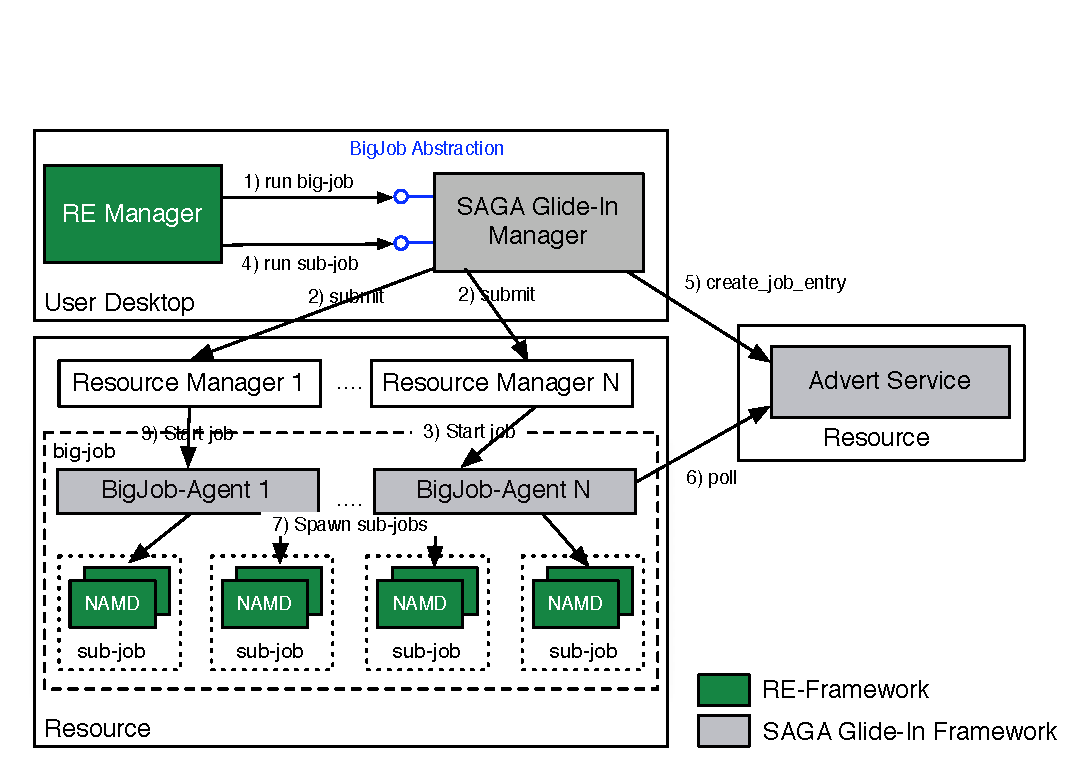
\includegraphics[width=0.82\textwidth]{../figures/Bigjob_arch.pdf}
          \caption{\footnotesize SAGA/BigJob Architecture
              }
      \label{fig:bigjob}
\end{figure}

Figure ~\ref{fig:bigjob} shows the architecture of SAGA BigJob.
It consists of three components: (i) the SAGA-BigJob Manager, (ii) the BigJob Agent and (iii) the advert service. The SAGA-BigJob manager submits the BigJobs to the resource manager and the sub-job descriptions to the \emph{advert server}. The advert server can be on any machine and is a central key/value store which is used for communication between the SAGA-BigJob Manager and the BigJob agent. There is a separate BigJob agent for each BigJob. Thus, every BigJob on every machine has a local BigJob agent. Once the BigJobs become active, the BigJob agent retrieves the job descriptions from the advert server, allocates the required number of nodes and launches the sub-jobs on each resource. The BigJob agent continuously monitors the running sub-jobs and updates the sub-job states in the advert server. Once a sub-job finishes running, the nodes are freed and marked as available. The BigJob agent periodically polls the advert server for new jobs.
\subsection{Replica-Exchange Manager}\label{repexmanager} 

\jhanote{Just a suggestion for the title}

\jhanote{Abhinav: This subsection should help the reader understand
  the basic and common elements of the RE Framework -- job submission,
  role of bigjob-agent, replica agent, replica-exchange manager etc
  etc}
  
  Synchronous RE is only implemented in a centralised manner, where the
simulation and all the replicas are managed by a master.  % \alnote{The
%   following needs refinement}\athotanote{any better now?}
Because there is a synchronization step at the end of each exchange
step, we believe it will not help even if the replicas are managed in
a decentralized manner. By decentralized, we mean a case where each of the replicas are are managed individually. But, in the case of asynchronous RE, we
implement it in both centralised and decentralised manner. %And, we see that the decentralised implementation is much more efficient than the centralised implementation.  The synchronous and asynchronous RE have been successfully deployed on production level infrastructure such as the Teragrid and LONI.


\subsubsection{Synchronous and Asynchronous (centralized) RE Manager}
The reason for grouping synchronous and asynchronous (centralized) RE Managers is that they are very similar in operation. They are both centralized implementations, where a master process has complete control over the replicas and the whole experiment. We first explain the synchronous RE Manager and then the asynchronous (centralized) RE Manager.

The RE Manager receives various data about each
replica, such as the state (running, done, etc.,), temeperature and
energy from the BigJob agent after each run and based on that makes
the exchanges. This is in addition to the typical management tasks
carried out by the SAGA-BigJob Manager.  \jhanote{This should be 
moved to the subsection\ref{repexmanager}.}
The control flow of the synchronous RE Manager can be seen in Figure~\ref{fig:coordination}a). While the figure actually shows the control-flow in the case of centralized asynchronous RE, since both the implementations are centralized, there is only a slight difference. First, The the RE Manager starts the BigJob. This is done by making the SAGA BigJob Manager submit a job request to the resource manager. While the job request may be in the queue, the RE Manager posts the job descriptions of each of the replicas to the advert server. The RE Manager also creates directories, configuration files and stages them to the respective directories. Once the resource manager allocates the resources, the BigJob becomes active. Then the SAGA BigJob Manager launches the BigJob agent. The BigJob agent obtains the list of nodes allocated by the resource manager. The BigJob agent retrieves the job descriptions from the advert server and writes nodefiles for each of the replicas and runs them. The BigJob agent also monitors the replicas and posts their current state the advert server. The RE Manager constantly queries the advert server for the latest replica states. When the RE Manager finds a replica that has finished running, it collects the energy and temperature of that replica by reading the output file. Once \emph{all} the replicas have finished running, the RE Manager makes the exchanges. The exchange is done by exchanging the temperatures and writing new configuration files. With the new configuration files in place, the RE Manager posts the job descriptions to the advert server. The BigJob agent finds the replicas and restarts them. The RE Manager counts the successful exchanges. This process is repeated until the required number of exchanges are done. 

The asynchronous (centralized) RE Manager is similar, if not identical to the synchronous RE Manager. The only difference is that instead waiting for \emph{all} replicas to finish running before making exchanges, the asynchronous (centralized) RE Manager, whenever it finds a replica that has finished running, it tries to find a partner to make and exchange and if successful, posts the job description of both the replicas to the advert server. It does does this in the following way. Figure~\ref{fig:coordination}a) shows the control-flow. Once the RE Manager finds a replica that has finished running, it goes through the states of all the other replicas. If it finds a partner, it makes the exchange. If not, it takes a step back, retrieves the states of all the replicas. It starts again and tries to find a replica that has finished running and if it finds one, it tries to find that replica a partner. The RE Manager counts the successful exchanges. This process is repeated till all the exchanges are made. 

Where as in the synchronous RE, all the exchanges happen at a time, when all the replicas are finished running. This could be counted as one exchange step or a generation. At each exchange step, the number of pairwise exchanges taking place is half the total number of replicas. In asynchronous RE, we count the number of pairwise exchanges. 

\subsubsection{Asynchronous (decentralized) RE Manager and the replica agent}

The asynchronous (decentralized) RE Manager is just the SAGA BigJob framework, almost without any added functionality. By decentralized, we mean a case where each of the replicas are are managed individually instead of a master managing all the replicas. The only additional thing that the RE Manager does is that it queries the advert server for the current exchange count and when all exchanges are done, kills the experiment. It does the basic things such as starting the BigJob, submitting the job descriptions of the replicas, staging files initially and starting the BigJob agent. Once the BigJob becomes active, the BigJob agent runs a \emph{replica agent} instead of a replica. The replica agent is just a wrapper script for the replica, which runs and manages the replica. The BigJob agent has nothing else to do after it launches the replica agent, because for the length of the experiment, the replica agent would be running and managing the replica. The replicas are restarted, when needed by the replica agent itself. 

Figure~\ref{fig:coordination}b) shows the decentralized control-flow. Each replica is managed by a unique replica agent. The replica agent upon launch runs the replica. It receives the nodefile from the BigJob agent. It then constantly monitors the replica and when the replica finishes its run, it updates the advert server with the current state of the replica. It also reads the temperature and energy from the output files and posts the values to the advert server. It then goes through the list of replicas and tries to find an exchange partner. If it finds another replica available, it re-verifies the states of both itself and the other replica and if it finds both still available, marks their states as "Pending". The replica that initiates the exchange is the replica in-charge of the exchange. It then exchanges their temperatures via the advert server. It then modifies its configuration files locally, sets its state as running and runs the replica. On the other hand, the other replica's state is not set as "Ready" and that makes the other replica's replica agent to retrieve its own temperature from the advert server, modify its configuration file locally and run the replica. If at all the negotiation fails or the exchange is unsuccessful, the process is repeated. The replica agent that initiated the exchange increments the exchange count by one. 


\section{Implementation of Synchronous and Asynchronous RE}

\jhanote{This section should help the reader understand the control
  flow - which is YOUR IMPLEMENTATION of the RE algorithm. Need to
  make reference to Figures 2a and 2b}

We present the implementation details of the synchronous RE and the
two implementations of the asynchronous RE algorithm here.

We are primarily interested in learning the scale-up and scale-out
properties of synchronous and asynchronous RE and hence are not
concerned by the queue wait time. % In the following, we will
% explain how we implement the synchronous RE simulations.

To be able to quantify the various terms involved, we will consider the
following configuration for a RE experiment. The total number of replicas ($N_R$) in the
ensemble are 32 and the total number of pairwise exchnges ($N_X$) is
128. That would mean 8 generations or 8 on a homogeneous
infrastructure 8 restarts per replica. The ensemble of replicas are run
concurrently. Our experiments are performed on LONI and Teragrid
shared resource \emph{QueenBee}. Each replica is configured to run 500
time-steps and is allocated 16 processors. It should be noted that we are
talking about the average values whenever we mention quantities. Each
replica takes 91 seconds to complete the 500 time-steps from a fresh
start and 68 seconds every time it is restarted. Thus, if each replica
is restarted 7 times, the average time per generation is 71
seconds. The total runtime of the ensemble of replicas concurrently
run would depend on the total number of times each the replica was
restarted. And in this case it is 8 and the total run time is $71
\times 8 = 568$ seconds.
Nanoscale molecular dynamics (NAMD) (Phillips et al.
2005), a highly scalable, parallel MD code, is used to carry out the MD simulation
corresponding to each replica run. It is important to mention that any other MD or
Monte Carlo code could be used just as simply and effectively.
% \jhanote{this should go} Also in this section, when we say replica, we
% mean NAMD. \jhanote{NAMD is just a piece of software!}

\subsection{Synchronous RE}


%The RE Manager first submits the BigJob to resource manager. \jhanote{
  %is this true of all 3 cases? if so, this should be in
  %subsection~\ref{repexmanager}} 
Once the BigJob is active, the BigJob agent writes a
nodefile for each replica and starts the jobs. And the average time
it takes to start one replica is 0.3 seconds. For 32 replicas, it is
9.6 seconds. For each pair of replicas, it is 9.6/16=0.6 seconds.

\jhanote{Remember: if the reader has not understood the control flow
  already, all this will not make sense!}

%While it is the case that the BigJob agent is ready to start the new
%replicas at the start of the first run of the simulation, it is not
%always the case. \jhanote{previous sentence is difficult to
  %understand} Once the BigJob agent starts the replicas, it also
%monitors them and updates the states in the advert server.  It also
%keeps a list of free and busy nodes. 
The BigJob agent takes 0.92 seconds to process a replica that is found to be done running.
That is the time it takes to update the state and mark the nodes as free. Therefore, while there is a gap of 9.6 seconds between the
start times of the first and last replica, there is a difference of
29.44 seconds between the end time of the first replica and the last
replica. This should be included in $T_W$. This also overlaps the
startup time. So we need not count the startup time.

The replicas are now running, and the RE Manager periodically queries
the advert server for the latest replica states and marks the replicas
which finish running as done. The RE Manager typically doesn't find
all the replicas as done exactly at the same time. This is because of
two reasons: (i) even though we are using a homogenous infrastructure,
we observed that replica run time varies by 1 or 2 seconds ($\delta$),
(ii) the additional time the BigJob agent takes at the end of the each
replica's run updating the data. And also, the RE Manager, once it
finds that a replica is done, retrieves the current energies and
temperatures by reading the output files. This takes 0.4 seconds per
replica and for 32 replicas, it is 12.8 seconds.  We are calling all
this time between end of runtime and start of exchange making $T_W$
and for 32 replicas it is approximately: 29.44+12.8=42.24
seconds. Since exchanges are done in pairs, for each pair it would be
42.24/16 = 2.64 seconds.

Since this is a synchronous RE, all the replicas finish running before
the exchanges are started. \jhanote{The previous sentence is an
  example of what needs to be already explained!}  Hence, the RE
manager won't spend any time searching for partners and $T_F$ is 0
seconds. $T_{ex}$ includes updating configuration files and
transferring the them to their respective directories, in this case,
locally. It takes 0.2 seconds to write and copy a file
locally. $T_{ex} = 0.2 \times 2=0.4$ seconds. $T_{coord}$ is the time
it takes to resubmit the pair of replicas to the advert server, which
is $0.11\times 2 = 0.22$ seconds. Therefore, $T_X$ is
$0+0.4+0.22=0.62$ seconds. 

If $T$ is the total to complete the RE experiement, and $p$ is
the probability of a successful exchange, quantifying equation
~\ref{eq:totaltime}, we get
\begin{eqnarray}
T=  {1 \over p} \times {[ 568+ (0.62 + 2.64)\times 128]} = {1 \over p} \times (990)
\label{eq:timebt}
\end{eqnarray}


%The BigJob agent also monitors the replicas it
%launched and posts the statuses of the replicas to the advert
%server. The master queries the advert server for the latest job states
%and when it finds that \emph{all} the replicas in the generation are
%'Done' ($T_{MD}+T_{W}$), it starts making the exchanges ($T_{X}$).
%\alnote{We should clearly differ between describing the coordination pattern and analyzing the time} $T_{X}$ is comprised of the time to find a partner $T_{F}$, exchanging states/file-staging $T_{ex}$ and status updates $T_{coord}$. \alnote{repetition with sec 2} After all the exchanges are done in a particular generation, the replica job descriptions are posted to the advert server and the BigJob agent restarts the replicas. This process is repeated until the required number of exchanges are made. The time to make one exchange would be: \begin{eqnarray} t &=&  {1 \over p} \times {[T_s+T_{MD} + T_{X} + T_{W}]}  \label{eq:sy} \end{eqnarray} where $p$ is the probability of a successful exchange.

%If the number of exchanges is ($N_{X}$), the total time to completion ($T_{C}$) would be:
%\begin{eqnarray}
%T_{C} &=& N_{X} \times t 
%\label{eq:synch}
%\end{eqnarray}
%If there are $\eta$ independent exchange events then the time $T$ for 
%N$_x$ exchanges is $T \over \eta$. For this synchronous RE model, 
%$\eta$ is 1\alnote{1 or 2?}, as all the exchanges are carried out 
%in a serial manner. Also, assuming $p$ is 1,\alnote{unrealistic} 
%$T =  [T_s+T_{MD} + T_{X} + T_{W}] \times N_{X}$.
%Quantifying each of the terms above with experimental values observed 
%on QueenBee, we have:
%\alnote{$T_{MD}$ is for what scenario?}
%$T_s = 1.5\,sec; T_{MD}=90\,sec; T_{X}=T_{F}+T_{ex}+T_{coord}=0.3+1+0.6=1.9\,sec; T_W=varies.$ 
%\alnote{$T_{F}$ == 0.3\,sec? independent of number replicas? 
%Do we have an average value of $T_{W}$ with respect to different
%number of replicas maybe incl. stddev? table?}
%The value of $T_W$ increases with the number of replicas, because 
%the gap between the time the first and last replicas are 
%started increases. 


% \begin{figure}[t]
%       \centering
%           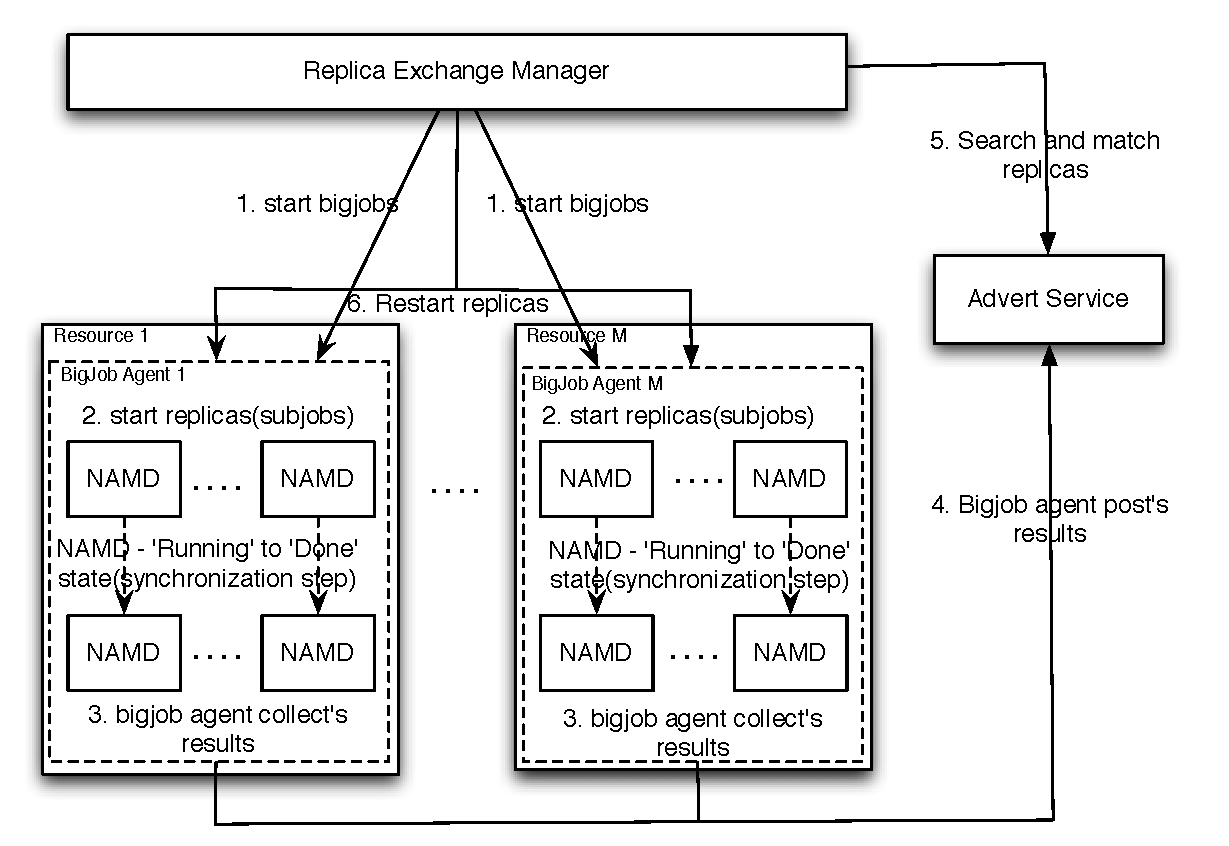
\includegraphics[width=0.8\textwidth]{synchronous.pdf}
%           \caption{\footnotesize Control Flow: Synchronous Replica Exchange
%               }
%       \label{fig:sync}
% \end{figure}

\begin{figure}%
\centering
\subfigure[Central]{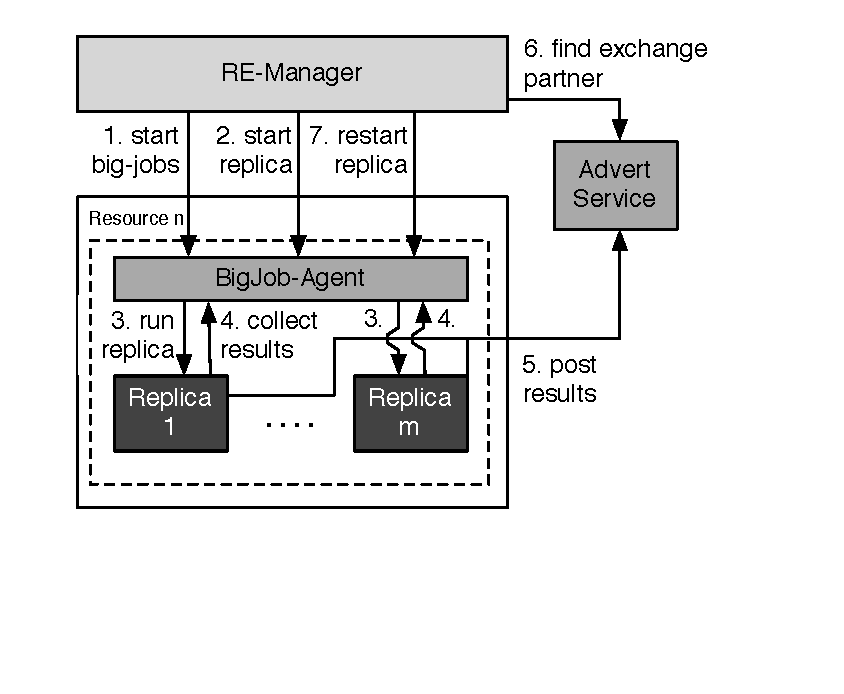
\includegraphics[width=0.47\textwidth]{../figures/central_AL.pdf}}\qquad
\subfigure[Decentral]{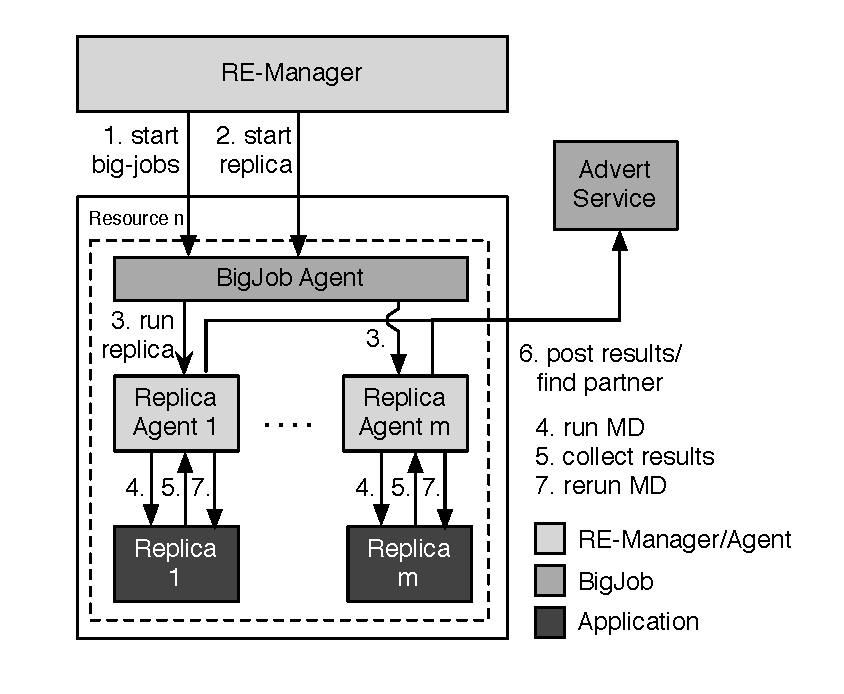
\includegraphics[width=0.47\textwidth]{../figures/decentral_AL.pdf}}\\
\caption{\textbf{Centralised vs. Decentralised Coordination:} Both
  central coordination style is used both by the synchronous RE (case
  I) and a version of the asynchronous RE (case II).  In the decentral
  style -- used by another version of the asynchronous RE (case III)--
  the master is only required for initially setting up all
  replicas. The later coordination is done peer-to-peer via the Advert
  Service.}
\label{fig:coordination}
\end{figure}


\subsection{Asynchronous (centralized) RE}
\alnote{please don't just copy paste. Only focus on the differences}


Here we describe the centralised
implementation.
 Once the BigJob is active, the BigJob agent writes a nodefile for
each replica and starts the repplicas. The average time it takes to
start one replica is 0.3 seconds. For 32 replicas, it is 9.6
seconds. Since $T_{MD}$ on a fresh run is 91 seconds, the BigJob agent
would be ready to restart the replicas by the time the RE Manager
submits to the advert server.

The replicas are now running, and the RE Manager constantly
queries the advert server for the latest replica states. Whenever the
RE Manager finds a replica in done state, it tries to find a partner
for the replica. The time to find the partner ($T_F$)
depends on $N_R$ and also on the number of replicas the RE Manager had
to sift through to finds an available replica. On average, RE Manager
will sift through $N_R/2$ replicas before it finds a partner. It
should be noted that we also implemented a special case for an ensemble containing a very large
number of replicas, where the RE Manager tries to find a
partner randomly. We observed that this only improves the performance
when the ensemble contains more than 128 replicas. It takes 0.01
seconds per query. Thus for 32 replicas, on average, $T_F$ is
$16\times 0.01=0.16 seconds. T_{ex}$ is the time it takes to update
the configuration files and copy them locally. That would be
$0.2\times 2=0.4 seconds.$ $T_{coord}$ is the time it takes to
resubmit the pair of replicas to the advert server, which is
$0.11\times 2 = 0.22$ seconds. Therefore, $T_X$ is
$0.16+0.4+0.22=0.78$ seconds. Therefore, on average, it takes 0.78
seconds for the RE Manager to make an exchange. For 16 exchanges, it
is 12.48 seconds.

As mentioned earlier, the BigJob agent takes 0.92 seconds to find that
a replica is done (1.84 for a pair), update the state and free the
nodes. Therefore it takes 29.44 seconds for 32 replicas. But even as
the first pair of replicas are marked as done by the BigJob agent, the
RE Manager concurrently makes the exchange between that pair of
replicas. The point we are trying to make is that the timelines of the
RE Manager and the BigJob agent run parallel to each other and there
also is a lot of overlap.  As the simulation progresses, instead of
all the replicas starting and ending together, groups or pairs of
replicas start and end at the same time.  Since the BigJob agent takes
longer to process the replicas, the RE Manager by then makes the
exchanges and resubmits the replicas to the advert server. The pairs
of replicas belonging to the first few exchanges might have waited the
29.44 seconds at the BigJob agent. But we observed that groups of
replicas belonging to the later exchanges wait for only half that
amount of time. That is 29.44/2 = 14.72. That would be 14.72/16 =0.92
for a pair of replicas. $T_W$ = 0.92 seconds.

%The point we are trying to make is that the BigJob agent might not be free while the RE Manager submits the replicas to be restarted. But as the experiment progresses, instead of all the replicas in the ensemble running in synchronization, pairs of replicas would start and end together. 
% By the time the BigJob agent finishes processing the last of the replicas that finished running, the RE Manager would have re-submitted 15 pairs of replicas to the advert server for restarting by the BigJob agent. In the next couple of seconds the rest of the replicas would have been exchanged and submitted to the advert server.

If $T$ is the average time between successful exchanges, and $p$ is
the probability of a successful exchange, Quantifying equation
~\ref{eq:totaltime}, we get
\begin{eqnarray}
T=  {1 \over p} \times {[568 + (0.78 + 0.92)\times 128]} = {1 \over p} \times 786 
\label{eq:timebt}
\end{eqnarray}


\subsection{Asynchronous (decentralized) RE}

The decentralised implementation is very different from the
implementation of cases I and II. Although the RE-Manager starts the
simulation and launches the BigJobs, each replica is managed by a replica agent.(see
Figure~\ref{fig:coordination}b)). %\jhanote{What is meant by a
%  decentralised manner?} 

Once BigJob become active, the BigJob agent starts the replica agents, 
the replica agents in turn start the replicas. It takes 0.3 seconds to start a replica-agent and 9.6 seconds to start 32 replica agents. 
The replica agents are now
running and each of them start their replica. The replica agent creates the output
and error files, reads the configuration and starts the replica. All
these actions, which are repeated after every exchange, take 1.3
seconds.

The replica agent constantly monitors the replica and when it finds
that the replica finished running, it updates its state in the advert
server, which takes 0.11 seconds and also retrieves the energy and
temperature from the output files, each of which actions takes 0.025
seconds. It then posts both these values to the advert server. Thus
$T_W$ is 1.3+0.4=1.7 seconds.

Then it tries to find a another replica to make an exchange. Each
replica agent tries to find a partner in a completely random
manner. This was necessitated by the fact that if all of the replica
agents tried to find a partner by going through the list of replicas
serially, there would be a lot of contention and even grid-lock. We
observed that on average, the replica agent makes 15 queries before it
finds a partner. Each query is 0.11 seconds, thus $T_F$ is 1.65
seconds. It should be noted here that in the centralized version of
asynchronous RE, where only 2 connections to the advert server existed
(RE Manager, BigJob agent), each query took only 0.01 seconds. But in
the decentralized version, since each replica agent maintains an open
connection to the advert server, there are 32+2=34 connections
open. This effects the performance of the advert server. Once the
replica agent finds another replica agent available, it re-verifies
it's own state and the other replica agent's state. If the replicas
are still available, the replica agent sets both the replica states as
"Pending". This is done to make sure that duplicate exchanges don't
take place. Now, the replica agent which initiated the exchange set's
the temperatures of both replicas in the advert server. The the master
replica agent sets both the states as ready, which means that the
control flow can move forward to updating the configuration files and
restarting the replicas. All this process takes on average 15 more
queries to the advert server. Thus, $T_{ex}$ is 1.65 seconds. It
should be noted here that the temperatures are exchanged over the
advert server and the replica agent writes a new configuration file
locally. This removes the need to stage the configuration files to
different machines. This is possible because there is a replica agent
for each replica locally. Where as earlier, the RE Manager and the
replica might be located on different machines. $T_{coord}$ is the
time it takes to update the state in the advert server, which is 0.11
seconds. Thus, $T_X$ is 1.65+1.65+0.11= 3.41seconds.

If $T$ is the average time between successful exchanges, and $p$ is
the probability of a successful exchange, quantifying equation
~\ref{eq:totaltime}, we get
\begin{eqnarray}
T=  {1 \over p} \times {568 + {(3.41+1.7)\times 128\over 16}} = {1 \over p} \times 609
\label{eq:timebt}
\end{eqnarray}


\alnote {one could ask why is the config file staged in case I and II
  then?}  Where as, in the other two implementations the exchanges
happen sequentially. But in the decentralised implementation, there
would be many pairs of replica agents negotiating the exchanges. It
should be noted that while this causes the time taken per unit
exchange to go up, more exchanges occur in unit time.

If there are $\eta$ independent exchange events then the time $T$ for
N$_X$ exchanges is $T \over \eta$. For this asynchronous centralized
RE model, $\eta$ is $N_R \over 2$, as at any time there could be a
maximum of $N_R \over 2$ pairs of replicas negotiating.  \alnote{We
  really need to discuss $\eta$ tomorrow on the call!}


The decentralised implementation depends on the advert server much
more than the other two implementations. Where as, in the other two
implementations there are only a handful of connections to the advert
server (one connection from each of the machines), in the
decentralised implementation, each replica agent has an open
connection to the advert server. If the number of replicas is 256,
then there would be approximately \jhanote{approximately or exactly
  256?} that many connections open with the advert server. This does
not seriously impact the communication times with the advert server,
and the overhead is unnoticeable.

Although both case II and case III implement the asynchronous RE
algorithm, they differ in the way they are implemented. The replicas
are either managed by a master (case II) or each replica is managed
individually (case III). We propose case III so as to not let the
master in case II become a bottleneck, which can happen very quickly
with a large number of replicas. \jhanote{If we believe this is the
  case then we need to document and show how/much the slow down with
  increasing replica is.} We do see in our experiments that the
decentralised implementation scales up and scales out better than the
other two implementations.

% \begin{figure}
% \centering
% %\subfigure[Control Flow: Decentralized Replica Exchange]{
% 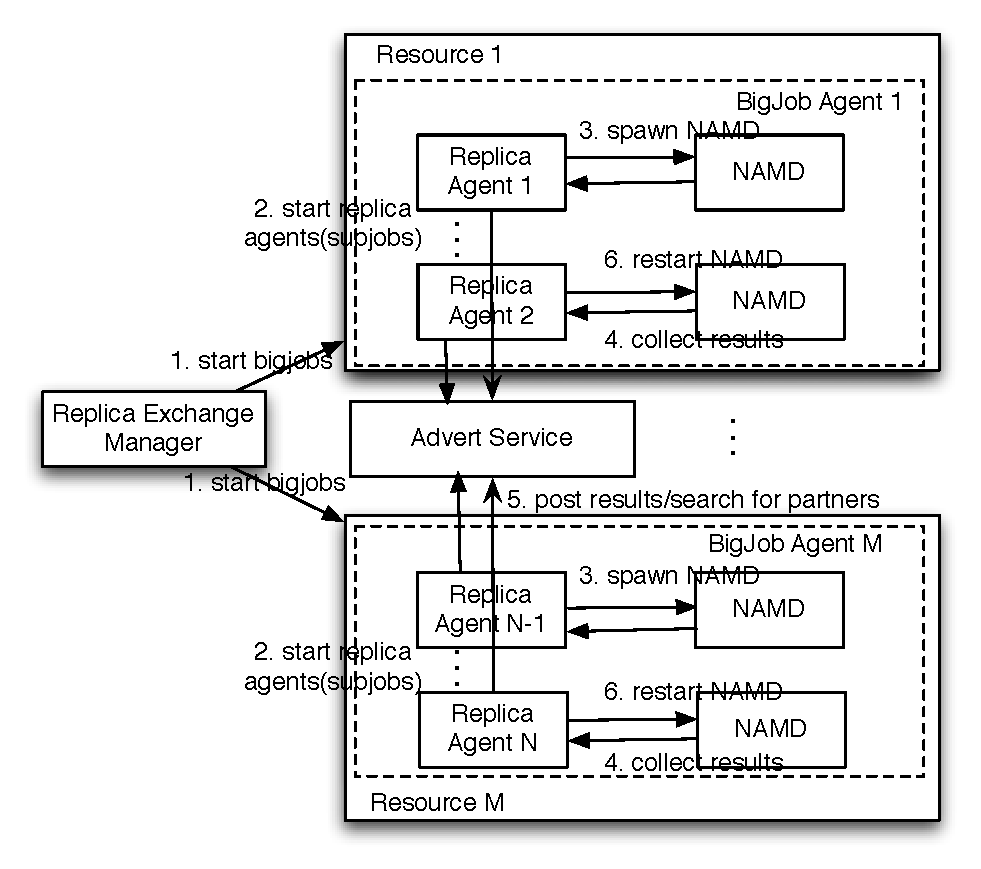
\includegraphics[width=0.9\textwidth]{asyncre.pdf}
% %\label{fig:async:b}
% \caption{\small Decentralized control flow: In the decentralized asynchronous RE, for  each replica there is a replica agent which individually manages the replica.}
% \label{fig:decent}
% %\vspace{-1em}
% \end{figure}

\alnote{we should write Case consistently with small or capital letter}
% We have to bear in mind that while Case II and Case III both implement the same asynchronous RE algorithm, they do it differently.
% At first glance it appears to be a question of philosophy, whether to
% let the replicas be managed by a master or to let each replica be
% managed individually.
%There could be implications effecting the performance of the
%algorithm. Where as in Case II, the master has to manage all the
%replicas and since it can only manage one replica at a time, although negligible, it is a cause for concern with large number of replicas. %The effect could be negligible and might now effect the overall performance.
%But the decentralized version (Case III) has no
%such issues as each replica is managed individually. % \jhanote{The distinction between Case 3 and 2 needs to
%  be made more clear. The following is ``implementation detail''. What
%  is the conceptual difference between Case 3 and Case 2?}

\section{Scale-Up and Scale-Out: Experiments and Results}

%
%%%%% FIGURE %%%%%
\begin{figure}
\centering
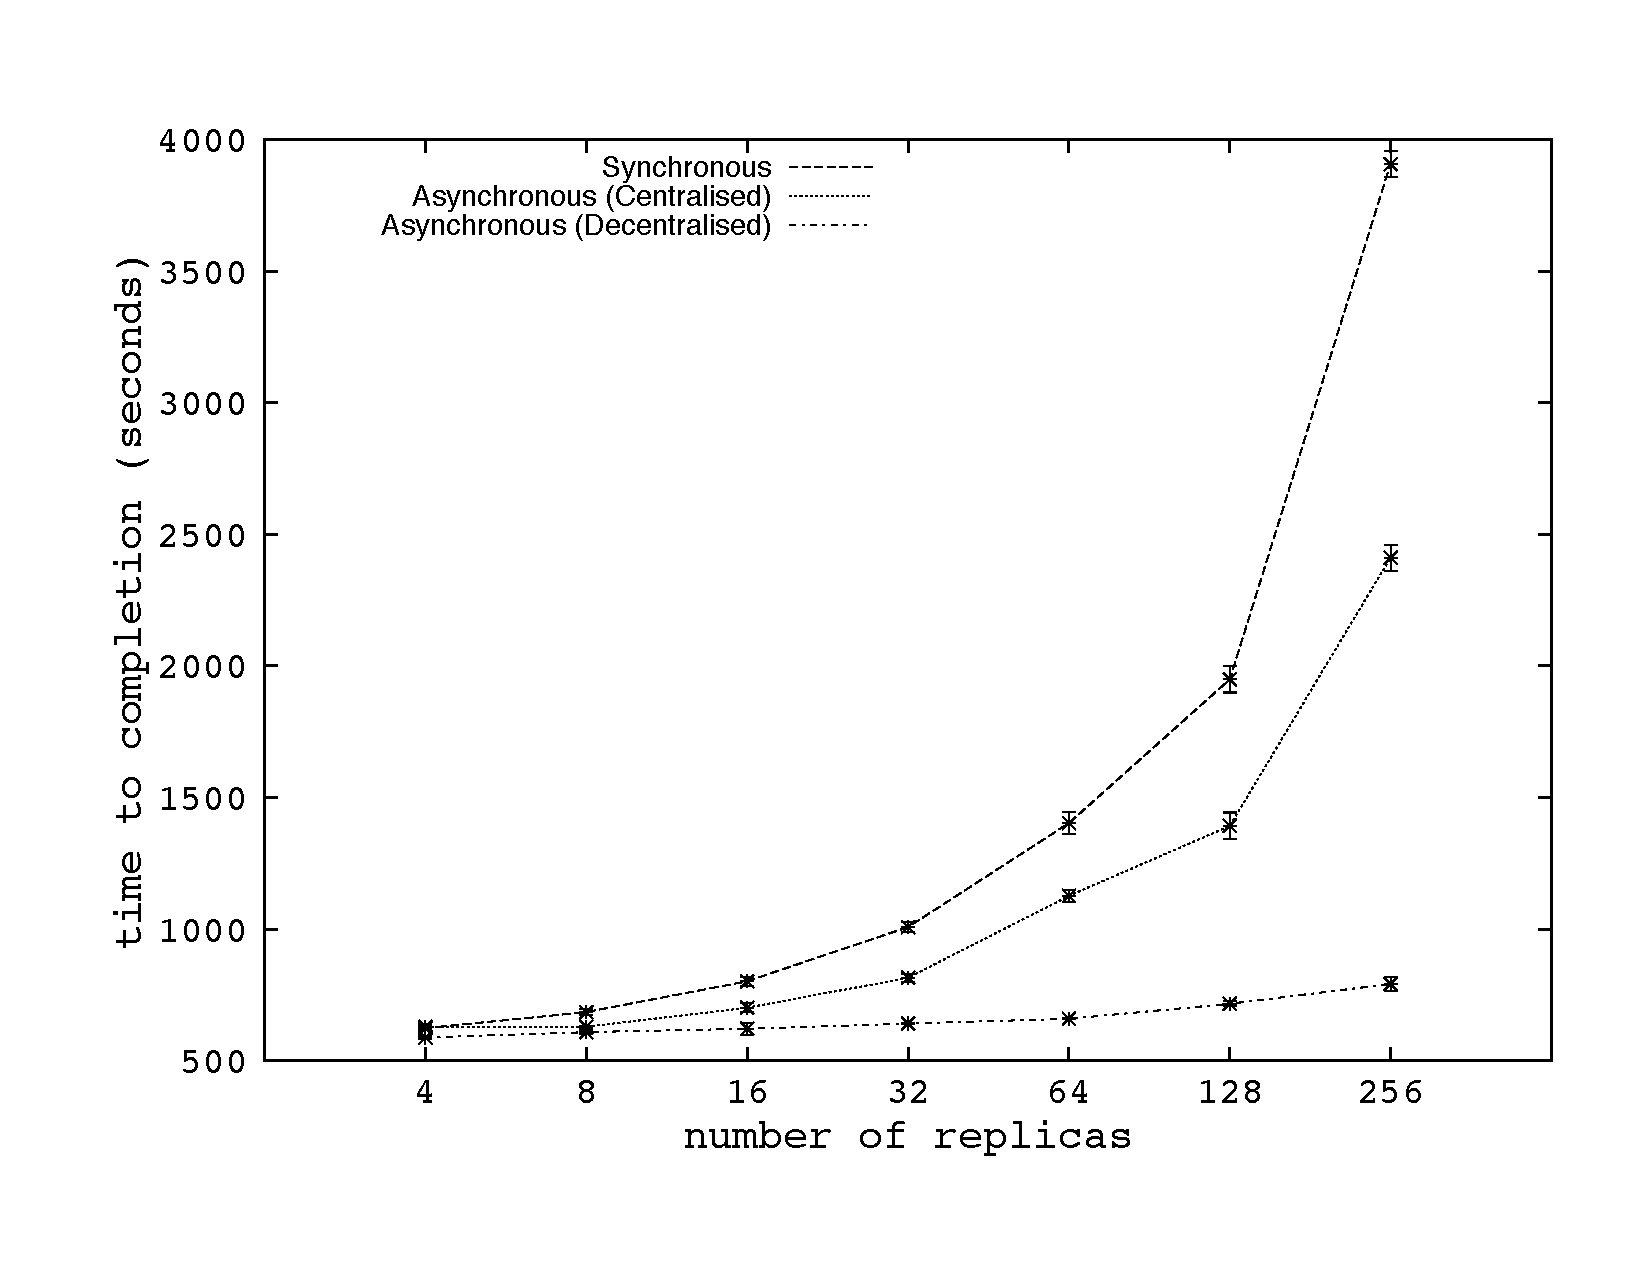
\includegraphics[width=0.9\textwidth]{../data/scale_up.pdf}
\caption{\small The graph shows the mean run times of synchronous and asynchronous - centralised/decentralised RE simulations on one machine. We repeated the experiments with up to 256 replicas. Up to 128 replicas, the experiments were conducted on QB and 256 replicas experiments were conducted on Ranger.}
\label{fig:graph}
\vspace{-1em}
\end{figure}

%While the traditional RE limits the exchanges to only neighboring temperatures, an asynchronous RE does not. This is not a concern when the number of replicas is small and there is little chance of an exchange between non-adjacent temperatures. However, as the number of replicas increases, the difference between the target temperatures becomes small enough to allow exchanges between non-adjacent temperatures. This also allows for 'crosswalks' to happen. The larger the number of crosswalks, the better is the performance of the simulation.

%To evaluate the performance of the various models of RE we have discussed in the abstract, we conducted several experiments on Teragrid and LONI resources. 
%In the following sentences we will analyze the performance of synchronous RE(Case I) with centralized asynchronous RE(Case II). 

\subsection{Scale-Up}

\subsubsection{Experiments}
In this section we describe the experiments we did increasing the number of replicas on a single machine. We configured the Cases I, II \& III to run parallel NAMD simulations with 4, 8, 16, 32, 64, 128 and 256 replicas sampling a temperature between 300 and 3000 K on Teragrid machines QueenBee and Ranger. \alnote{What resource?} In each simulation, one BigJob is launched with sufficient cores while each replica uses 16 MPI processes and runs 500 time steps between exchange attempts. Up to 128 replicas, all simulations were conducted on QueenBee, but the 256 replica simulations were conducted on Ranger as QueenBee allocates a maximum of 2048 cores per job. The metric used for comparison of 4, 8, 16, 32, 64, 128 and 256 replicas is the time to complete 16, 32, 64, 128, 256, 512 and 1024 attempted exchanges, respectively. It should be noted that the ratio between the number of replicas and the number of attempted exchanges is kept constant, for the purpose of comparison between each of these cases. It means that we are keeping the number of times each replica restarts, approximately, a constant. 

The mean run time is obtained by subtracting the queue wait time of the BigJob from the total time. As the ratio between the number of replicas and number of exchanges is kept constant, ideally, the runtime must remain constant too. In the graph (Figure~\ref{fig:graph}), we see an increase in the time to completion as the number of replicas increases. The increase in the completion time is not uniform across the three cases. We see the most slow down in case I and the least in case III.

\subsubsection{Scale up performance: Results and Analysis}

{\it Results:}\\

{\it Analysis: } From the graph (Figure~\ref{fig:graph}), we see that
Case I does not scale very well when we increase the number of
replicas. This is due to an inability to start and end all the
replicas at the same time and also due to the centralized control of the workflow. With more and more replicas, the time to start the replicas increases  and 
synchronization cost tends to increase too.  In Case II, the exchanges happen in
an asynchronous manner, but they are still conducted by the master
alone. As the number of replicas increases, the master quickly becomes
a bottleneck. But in Case III, the exchanges are all carried out in a
decentralised manner. Many exchanges can occur between different pairs
of replicas at the same time. Therefore, we say that the asynchronous
RE algorithm scales better and that the decentralised implementation
is better than the centralised implementation.

%
%%%%% FIGURE %%%%%
\begin{figure}
\centering
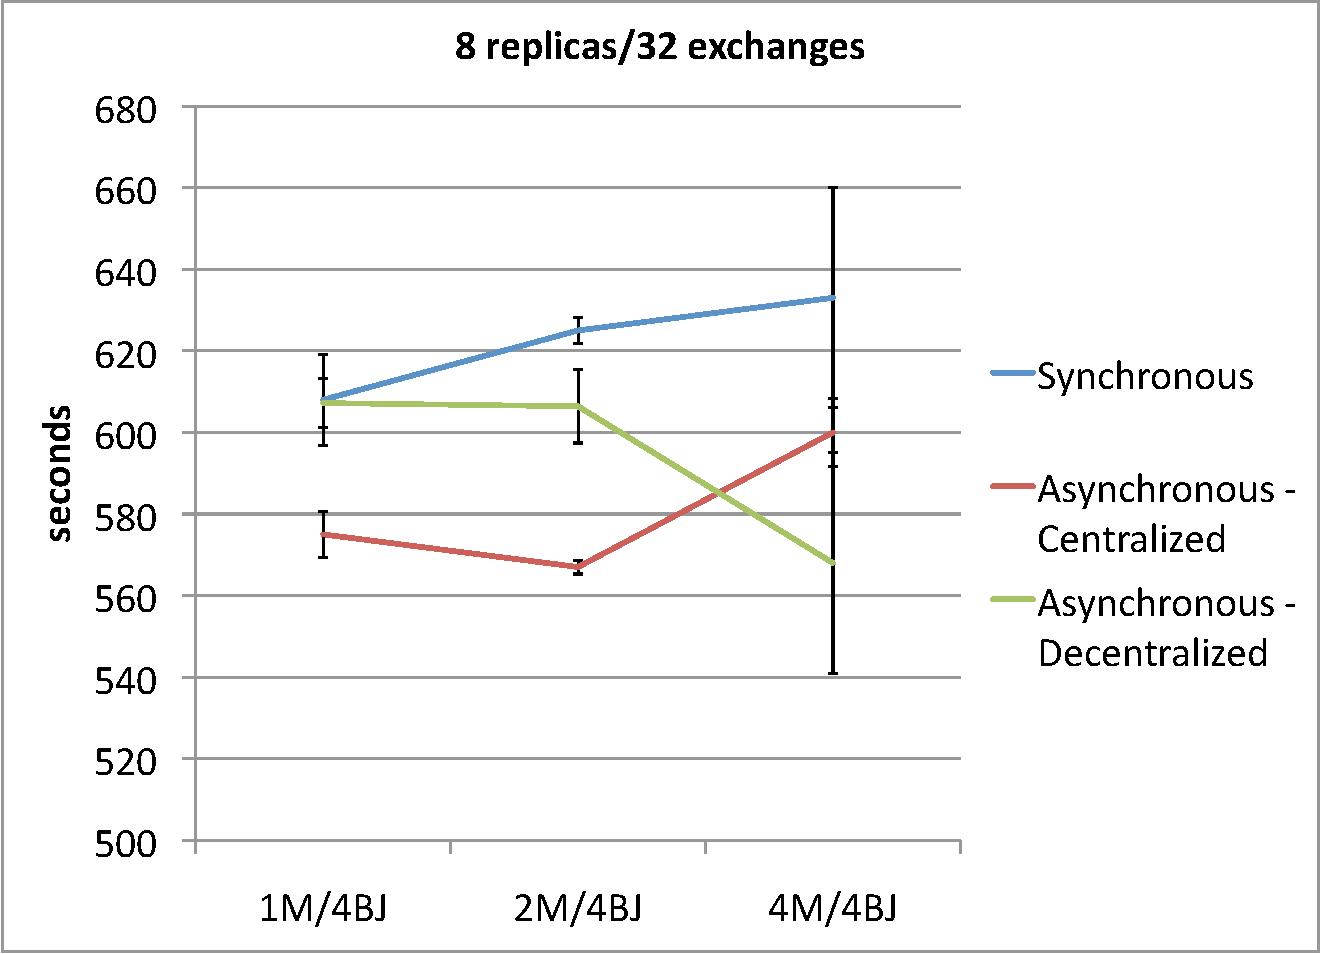
\includegraphics[width=0.9\textwidth]{../data/8rep.pdf}
\caption{\small The graph shows the mean run times of synchronous and
  asynchronous - centralised/decentralised RE simulations across two
  and four machines.}
\label{fig:2machines}
\vspace{-1em}
\end{figure}

\begin{figure}
\centering
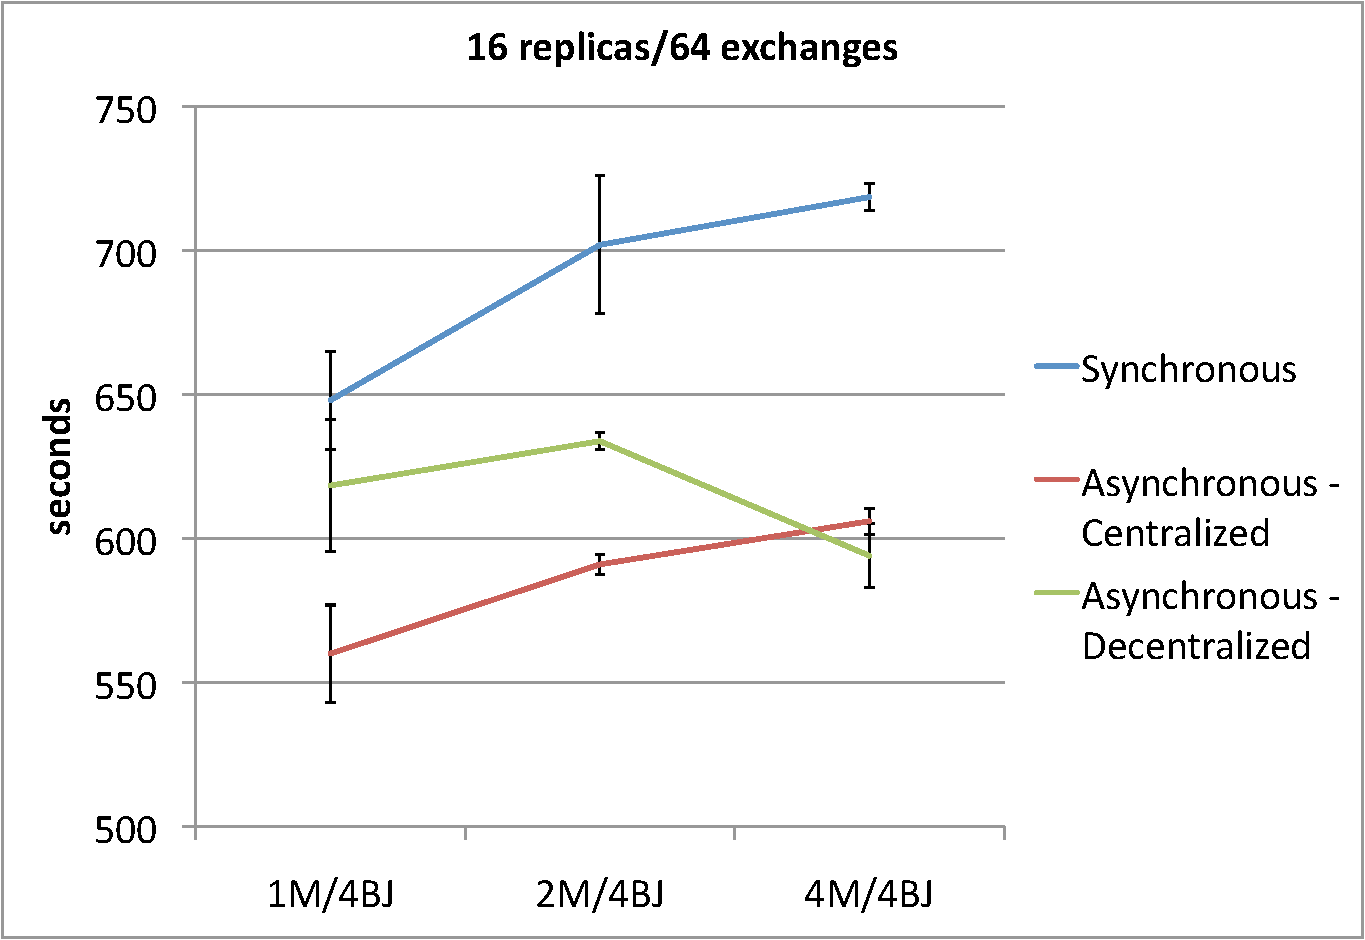
\includegraphics[width=0.9\textwidth]{../data/16rep.pdf}
\caption{\small The graph shows the mean run times of synchronous and
  asynchronous - centralised/decentralised RE simulations across two
  and four machines.}
\label{fig:2machines}
\vspace{-1em}
\end{figure}

\begin{figure}
\centering
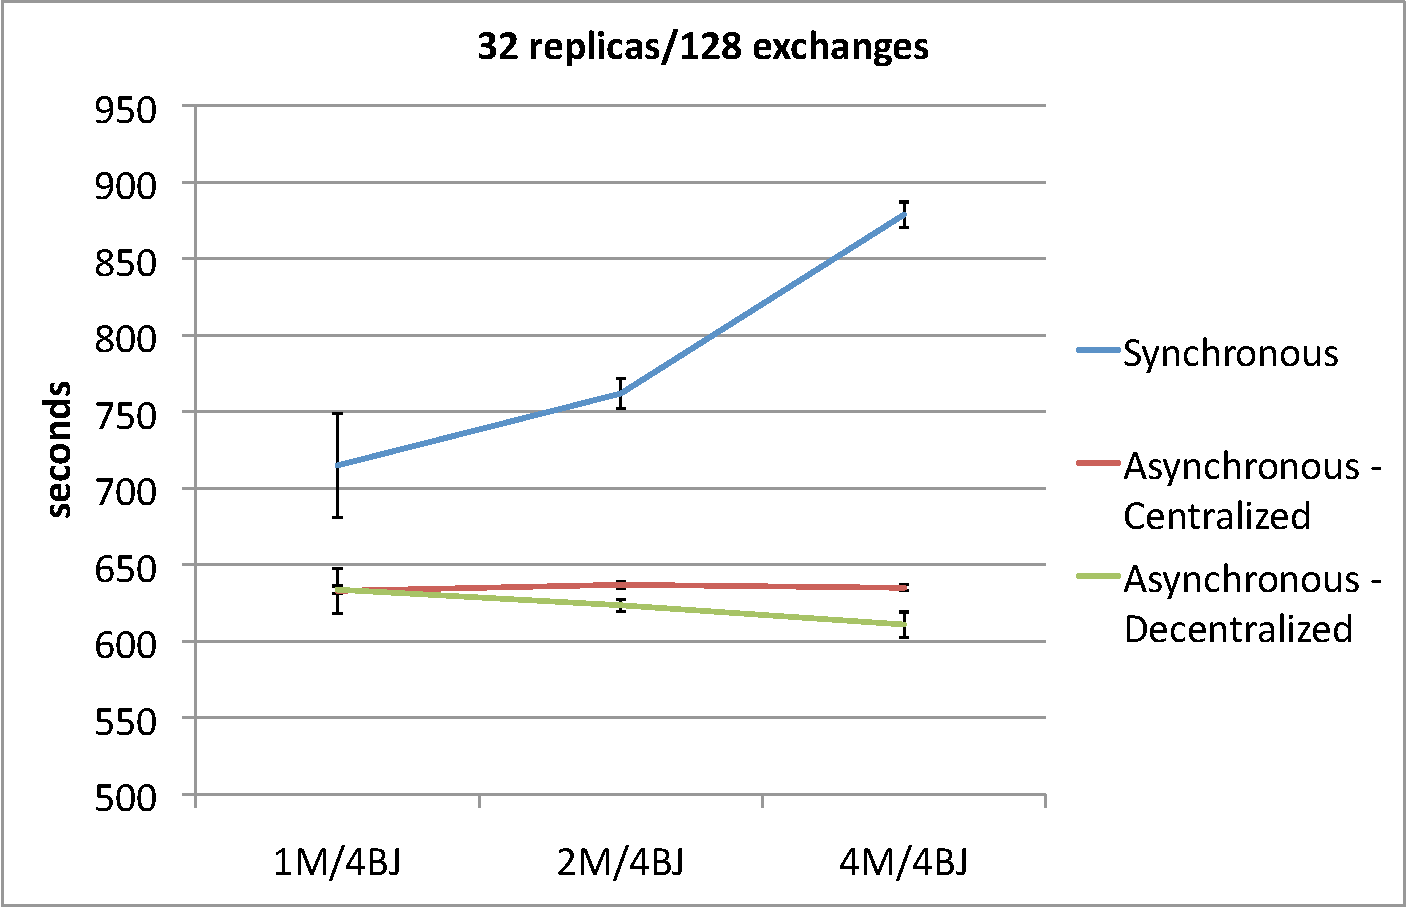
\includegraphics[width=0.9\textwidth]{../data/32rep.pdf}
\caption{\small The graph shows the mean run times of synchronous and
  asynchronous - centralised/decentralised RE simulations across two
  and four machines. }
\label{fig:2machines}
\vspace{-1em}
\end{figure}

\subsection{Scale out}

\subsubsection{Experiments}
In this section, we describe the experiments we did while increasing
the number of machines across which the experiments were done. We
chose LONI and Teragrid machines to run the experiments. We did
experiments distributed across two and four machines with 8, 16 and 32
replicas distributed equally across the machines.
Figure~\ref{fig:2machines} and Figure~\ref{fig:4machines} show the
behavior of Cases I, II and III across one, two and four machines,
respectively. Overall, there is not much difference between the local
and distributed runs in any case. The reason being that there is very
little interaction between the replicas. A very small configuration
file is staged to the remote machines after an exchange, which will
not add more than a couple of seconds per exchange. The rest of the
co-ordination is done via the advert service, which is usually located
on a remote machine in any case. Each query to the advert server is in
the order of milli seconds and does not produce a noticeable effect on
the performance.

\jhanote{There are several parts of the above paragraph that should be
  in the results sub-section. Similarly, there are parts in the
  experiments section for 'scale-up' that should be in the results
  section}

\subsubsection{Scale out performance: Results and Analysis}

{\it Results:}\\


{\it Analysis: } In Figure~\ref{fig:2machines}, we see the performance of all three cases when run in a distributed manner across two machines. As the data that is exchanged between replicas is very small, the Cases I, II and III behave in a similar manner to the way they behave on a single machine. \alnote{we should add some numbers and maybe a graph for an example scenario: x: machines y: time-to-solution} Again, asynchronous RE is better suited for distributed runs and the decentralised implementation scales best. The reason is, since each replica has its own replica agent, there is no need to transfer any files between machines. The required configuration files are created locally by the replica agent.


%In Case I, the pair-wise replica exchange can occur only between replicas of the same generation. Therefore, each exchange step is attempted only after all the replicas have finished running. After the exchange, all the replicas are restarted sequentially. This inserts a delay between the start time of the first replica, the last replica and the replicas in between. %As more resources become available at different times, the replicas already running or done are forced to wait for the newly running replicas to finish before moving on to the next exchange step. %Each exchange step is counted as an exchange.
%In Case II, the pair-wise replica exchange can take place between any two replicas in the ensemble irrespective of generation. As more resources become available, the new replicas join the ensemble immediately and the replicas already running are not restrained from attempting exchanges or restarting. This gives the asynchronous or synchronous RE a slight advantage. But with a large number of replicas we could easily see large difference.
%\athotanote{Further, we show performance gains by running across more than one machine. By running across more than one machine, we demonstrate the ability to divide the jobs into smaller sub-jobs and then distribute them across a number of machines, thereby reducing the risk of long queue wait times on an over-crowded resource. In Figure~\ref{fig:graph}, it can be seen that the asynchronous RE time to completion improves almost by a factor of 3 when moving from one machine to four machines. This was caused due to the fact that when the experiment was done on one machine, by the time the experiment ended, only 64 cores were allocated by the resource manager. But on the other hand, when the experiment was launched across four machines, it received an allocation of 64 cores on each of the four resources. The improvement that is seen in the case of synchronous RE from one to four machines is also due to a similar reason.} %The asynchronous RE appears faster by a couple of minutes due to the fact that when the BigJobs become available randomly, the synchronous RE has to wait for the newly running replicas to finish.

%slightly over 2 machines, but again increases over 4 machines. This is due to the fact that the experiments have been run only a handful of times but, over time, it can be assumed that it will result in reduced queue wait times.

\section{Conclusion}



%\athotanote{is this right? }
% We are also going to have a wider group of replicas to look at for
% each replica as we are not pairing the replicas.

% Also, we have the usual advantages of using a pilot-job,
% such as reduced queue wait times by not having to submit to the queue
% at every step.  We also provide major advantages when compared to
% Parashar et al.

%  to run the asynchronous RE simulations,
% including the ability to run MPI
% jobs.
% ??We need to evaluate the performance of our models and compare with other models for conducting replica exchange simulations.


%%%%% FIGURE %%%%%
%\begin{figure}
%\centering
%\subfigure[Time to complete 64 exchanges on QB with two 64 core BigJobs and on both QB/Louie jointly with a 64 core BigJob on each machine.]{
%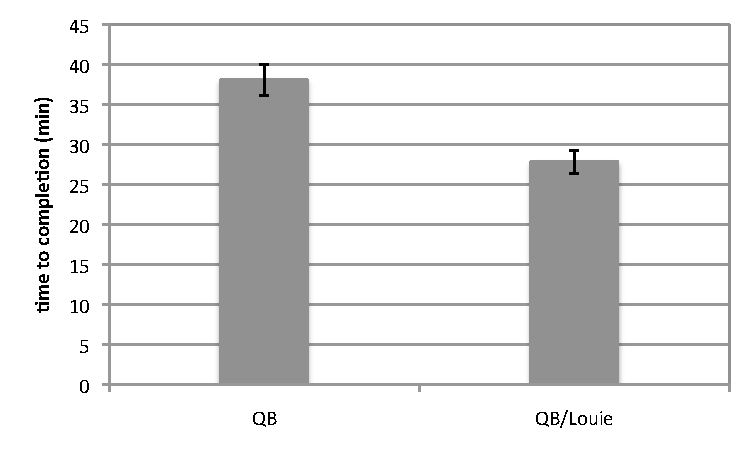
\includegraphics[width=0.40\textwidth]{figures/graph1.pdf}
%\label{fig:subfig3}
%}
%\hspace{0.5cm}
%\subfigure[Time to complete different number of exchanges on QB/Louie with a 64 core BigJob on each machine.]{
%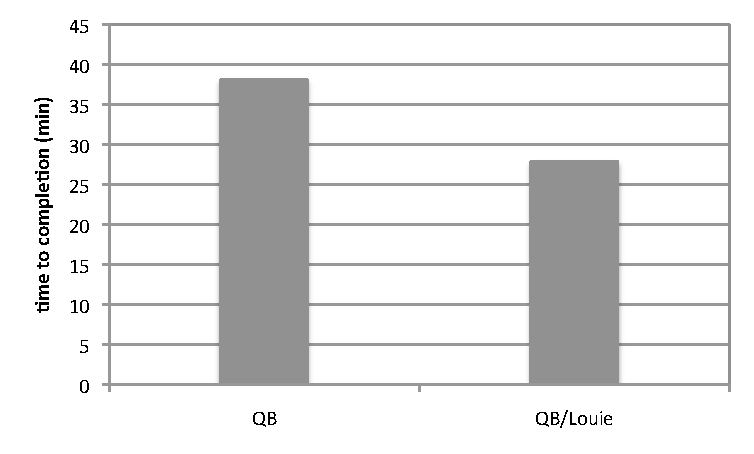
\includegraphics[width=0.40\textwidth]{figures/graph2.pdf}
%\label{fig:subfig4}
%}
%\caption{\small In Figure 2(a), we can see the improvement in performance when run on more than one machine. It is due to the fact that usually the first queued job becomes active before the second on a machine and running jobs on more than one machine solves this problem. In Figure 2(b), we can see consistent performance over prolonged runs, making 32, 64 and 128 exchanges.}
%\label{fig:graphs}
%\vspace{-1em}
%\end{figure}
%%%%% FIGURE %%%%%

An important motivation for this work is to implement a scheme that does not depend on a
static, well defined model of resource availability. %We test and scale
%our implementation on production level grids such as Teragrid and
%LONI~\citep{LONI_web}.
Preliminary results, shown in Figure~\ref{fig:graph}, indicate the
most important advantages of asynchronous RE and SAGA/BigJob over
traditional RE: (a) allows for exchanges to occur between replicas
with non-nearest temperatures, which in turn allows crosswalks to
happen (b) a reduced time to completion when running on more than one
machine due to improved resource availabilities, (c) the advantage of
using a pilot-job mechanism, which eliminates the waiting times at the
local resource manager, \alnote{have shown this in prev. papers, but
  we don't really have data in this one} and (d) the ability to scale
out across different production level infrastructure, such as, the
Teragrid and LONI.
% It performs well even after doubling and quadrupling the number of
% exchanges required to complete the simulation. The time to
% completion only increases by 35\% after doubling and 117\% after
% quadrupling the number of exchanges.
%\athotanote{should the results
%  be included in the conclusion or in a separate results section? Do
%  you agree with the \# of exchanges scheme to show the data?}
% Unfortunately we have results only for Case II currently, but 

%In summary, we have established the ability to scale-out across different
%infrastructure and compared the performance of the asynchronous
%RE with the synchronous RE at large scales. 
Further, we compare the traditional RE model (case I) and the centralised (case II) and decentralised (case III) models of the asynchronous replica exchange by modeling and repeating the experiments a reasonable number of times, so as to accurately quantify the scientific and performance gains. %We also propose to measure the frequency with which crosswalks occur with increasing number of replicas and measure the advantages due to a decentralized implementation in the full paper.


%With this asynchronous replica exchange mechanism we can improve the
%number of exchanges per unit time, a key parameter in judging the
%performance of a replica-exchange mechanism. \athotanote{is this
 % right? }  We are also going to have a wider group of replicas to
%look at for each replica as we are not pairing the replicas. Also, we
%have the usual advantages of using a pilot-job, such as reduced queue
%wait times by not having to submit to the queue.  Unfortunately we
%dont have results \jhanote{What results can we present -- any? some?},
%so we will say, (i) we establish the ability to scale-out (distributed
%and exa-scale) across different infrastructure (ii) compare the Async
%versus sync formulation at unprecedented scales \jhanote{At least
%  outline what infrastructure we / you are planning to use?} (iii)
%compare different implementations of the Async version
 

\begin{acknowledgement}
  This work is part of the Cybertools (http://cybertools .loni.org)
  project and primarily funded by NSF/LEQSF (2007-10)-CyberRII-01.
  Important funding for SAGA has been provided by the UK EPSRC grant
  number GR/D0766171/1 (via OMII-UK) and HPCOPS NSF-OCI 0710874. This
  work has also been made possible thanks to computer resources
  provided by TeraGrid TRAC TG-MCB090174 and LONI resources.
\end{acknowledgement}

\bibliographystyle{kluwer}
\bibliography{saga,literature}    
\end{document}

